% Options for packages loaded elsewhere
\PassOptionsToPackage{unicode}{hyperref}
\PassOptionsToPackage{hyphens}{url}
\PassOptionsToPackage{dvipsnames,svgnames,x11names}{xcolor}
%
\documentclass[
  letterpaper,
  DIV=11,
  numbers=noendperiod]{scrartcl}

\usepackage{amsmath,amssymb}
\usepackage{lmodern}
\usepackage{iftex}
\ifPDFTeX
  \usepackage[T1]{fontenc}
  \usepackage[utf8]{inputenc}
  \usepackage{textcomp} % provide euro and other symbols
\else % if luatex or xetex
  \usepackage{unicode-math}
  \defaultfontfeatures{Scale=MatchLowercase}
  \defaultfontfeatures[\rmfamily]{Ligatures=TeX,Scale=1}
\fi
% Use upquote if available, for straight quotes in verbatim environments
\IfFileExists{upquote.sty}{\usepackage{upquote}}{}
\IfFileExists{microtype.sty}{% use microtype if available
  \usepackage[]{microtype}
  \UseMicrotypeSet[protrusion]{basicmath} % disable protrusion for tt fonts
}{}
\makeatletter
\@ifundefined{KOMAClassName}{% if non-KOMA class
  \IfFileExists{parskip.sty}{%
    \usepackage{parskip}
  }{% else
    \setlength{\parindent}{0pt}
    \setlength{\parskip}{6pt plus 2pt minus 1pt}}
}{% if KOMA class
  \KOMAoptions{parskip=half}}
\makeatother
\usepackage{xcolor}
\setlength{\emergencystretch}{3em} % prevent overfull lines
\setcounter{secnumdepth}{5}
% Make \paragraph and \subparagraph free-standing
\ifx\paragraph\undefined\else
  \let\oldparagraph\paragraph
  \renewcommand{\paragraph}[1]{\oldparagraph{#1}\mbox{}}
\fi
\ifx\subparagraph\undefined\else
  \let\oldsubparagraph\subparagraph
  \renewcommand{\subparagraph}[1]{\oldsubparagraph{#1}\mbox{}}
\fi

\usepackage{color}
\usepackage{fancyvrb}
\newcommand{\VerbBar}{|}
\newcommand{\VERB}{\Verb[commandchars=\\\{\}]}
\DefineVerbatimEnvironment{Highlighting}{Verbatim}{commandchars=\\\{\}}
% Add ',fontsize=\small' for more characters per line
\usepackage{framed}
\definecolor{shadecolor}{RGB}{241,243,245}
\newenvironment{Shaded}{\begin{snugshade}}{\end{snugshade}}
\newcommand{\AlertTok}[1]{\textcolor[rgb]{0.68,0.00,0.00}{#1}}
\newcommand{\AnnotationTok}[1]{\textcolor[rgb]{0.37,0.37,0.37}{#1}}
\newcommand{\AttributeTok}[1]{\textcolor[rgb]{0.40,0.45,0.13}{#1}}
\newcommand{\BaseNTok}[1]{\textcolor[rgb]{0.68,0.00,0.00}{#1}}
\newcommand{\BuiltInTok}[1]{\textcolor[rgb]{0.00,0.23,0.31}{#1}}
\newcommand{\CharTok}[1]{\textcolor[rgb]{0.13,0.47,0.30}{#1}}
\newcommand{\CommentTok}[1]{\textcolor[rgb]{0.37,0.37,0.37}{#1}}
\newcommand{\CommentVarTok}[1]{\textcolor[rgb]{0.37,0.37,0.37}{\textit{#1}}}
\newcommand{\ConstantTok}[1]{\textcolor[rgb]{0.56,0.35,0.01}{#1}}
\newcommand{\ControlFlowTok}[1]{\textcolor[rgb]{0.00,0.23,0.31}{#1}}
\newcommand{\DataTypeTok}[1]{\textcolor[rgb]{0.68,0.00,0.00}{#1}}
\newcommand{\DecValTok}[1]{\textcolor[rgb]{0.68,0.00,0.00}{#1}}
\newcommand{\DocumentationTok}[1]{\textcolor[rgb]{0.37,0.37,0.37}{\textit{#1}}}
\newcommand{\ErrorTok}[1]{\textcolor[rgb]{0.68,0.00,0.00}{#1}}
\newcommand{\ExtensionTok}[1]{\textcolor[rgb]{0.00,0.23,0.31}{#1}}
\newcommand{\FloatTok}[1]{\textcolor[rgb]{0.68,0.00,0.00}{#1}}
\newcommand{\FunctionTok}[1]{\textcolor[rgb]{0.28,0.35,0.67}{#1}}
\newcommand{\ImportTok}[1]{\textcolor[rgb]{0.00,0.46,0.62}{#1}}
\newcommand{\InformationTok}[1]{\textcolor[rgb]{0.37,0.37,0.37}{#1}}
\newcommand{\KeywordTok}[1]{\textcolor[rgb]{0.00,0.23,0.31}{#1}}
\newcommand{\NormalTok}[1]{\textcolor[rgb]{0.00,0.23,0.31}{#1}}
\newcommand{\OperatorTok}[1]{\textcolor[rgb]{0.37,0.37,0.37}{#1}}
\newcommand{\OtherTok}[1]{\textcolor[rgb]{0.00,0.23,0.31}{#1}}
\newcommand{\PreprocessorTok}[1]{\textcolor[rgb]{0.68,0.00,0.00}{#1}}
\newcommand{\RegionMarkerTok}[1]{\textcolor[rgb]{0.00,0.23,0.31}{#1}}
\newcommand{\SpecialCharTok}[1]{\textcolor[rgb]{0.37,0.37,0.37}{#1}}
\newcommand{\SpecialStringTok}[1]{\textcolor[rgb]{0.13,0.47,0.30}{#1}}
\newcommand{\StringTok}[1]{\textcolor[rgb]{0.13,0.47,0.30}{#1}}
\newcommand{\VariableTok}[1]{\textcolor[rgb]{0.07,0.07,0.07}{#1}}
\newcommand{\VerbatimStringTok}[1]{\textcolor[rgb]{0.13,0.47,0.30}{#1}}
\newcommand{\WarningTok}[1]{\textcolor[rgb]{0.37,0.37,0.37}{\textit{#1}}}

\providecommand{\tightlist}{%
  \setlength{\itemsep}{0pt}\setlength{\parskip}{0pt}}\usepackage{longtable,booktabs,array}
\usepackage{calc} % for calculating minipage widths
% Correct order of tables after \paragraph or \subparagraph
\usepackage{etoolbox}
\makeatletter
\patchcmd\longtable{\par}{\if@noskipsec\mbox{}\fi\par}{}{}
\makeatother
% Allow footnotes in longtable head/foot
\IfFileExists{footnotehyper.sty}{\usepackage{footnotehyper}}{\usepackage{footnote}}
\makesavenoteenv{longtable}
\usepackage{graphicx}
\makeatletter
\def\maxwidth{\ifdim\Gin@nat@width>\linewidth\linewidth\else\Gin@nat@width\fi}
\def\maxheight{\ifdim\Gin@nat@height>\textheight\textheight\else\Gin@nat@height\fi}
\makeatother
% Scale images if necessary, so that they will not overflow the page
% margins by default, and it is still possible to overwrite the defaults
% using explicit options in \includegraphics[width, height, ...]{}
\setkeys{Gin}{width=\maxwidth,height=\maxheight,keepaspectratio}
% Set default figure placement to htbp
\makeatletter
\def\fps@figure{htbp}
\makeatother

\KOMAoption{captions}{tableheading}
\makeatletter
\makeatother
\makeatletter
\makeatother
\makeatletter
\@ifpackageloaded{caption}{}{\usepackage{caption}}
\AtBeginDocument{%
\ifdefined\contentsname
  \renewcommand*\contentsname{Table of contents}
\else
  \newcommand\contentsname{Table of contents}
\fi
\ifdefined\listfigurename
  \renewcommand*\listfigurename{List of Figures}
\else
  \newcommand\listfigurename{List of Figures}
\fi
\ifdefined\listtablename
  \renewcommand*\listtablename{List of Tables}
\else
  \newcommand\listtablename{List of Tables}
\fi
\ifdefined\figurename
  \renewcommand*\figurename{Figure}
\else
  \newcommand\figurename{Figure}
\fi
\ifdefined\tablename
  \renewcommand*\tablename{Table}
\else
  \newcommand\tablename{Table}
\fi
}
\@ifpackageloaded{float}{}{\usepackage{float}}
\floatstyle{ruled}
\@ifundefined{c@chapter}{\newfloat{codelisting}{h}{lop}}{\newfloat{codelisting}{h}{lop}[chapter]}
\floatname{codelisting}{Listing}
\newcommand*\listoflistings{\listof{codelisting}{List of Listings}}
\makeatother
\makeatletter
\@ifpackageloaded{caption}{}{\usepackage{caption}}
\@ifpackageloaded{subcaption}{}{\usepackage{subcaption}}
\makeatother
\makeatletter
\@ifpackageloaded{tcolorbox}{}{\usepackage[many]{tcolorbox}}
\makeatother
\makeatletter
\@ifundefined{shadecolor}{\definecolor{shadecolor}{rgb}{.97, .97, .97}}
\makeatother
\makeatletter
\makeatother
\ifLuaTeX
  \usepackage{selnolig}  % disable illegal ligatures
\fi
\IfFileExists{bookmark.sty}{\usepackage{bookmark}}{\usepackage{hyperref}}
\IfFileExists{xurl.sty}{\usepackage{xurl}}{} % add URL line breaks if available
\urlstyle{same} % disable monospaced font for URLs
\hypersetup{
  pdftitle={TF binding analysis \textbar{} Using Enformer and IMPACT},
  pdfauthor={Temi},
  colorlinks=true,
  linkcolor={blue},
  filecolor={Maroon},
  citecolor={Blue},
  urlcolor={Blue},
  pdfcreator={LaTeX via pandoc}}

\title{TF binding analysis \textbar{} Using Enformer and IMPACT}
\author{Temi}
\date{}

\begin{document}
\maketitle
\ifdefined\Shaded\renewenvironment{Shaded}{\begin{tcolorbox}[breakable, borderline west={3pt}{0pt}{shadecolor}, enhanced, frame hidden, boxrule=0pt, sharp corners, interior hidden]}{\end{tcolorbox}}\fi

\renewcommand*\contentsname{Table of contents}
{
\hypersetup{linkcolor=}
\setcounter{tocdepth}{3}
\tableofcontents
}
\begin{Shaded}
\begin{Highlighting}[]
\NormalTok{knitr}\SpecialCharTok{::}\NormalTok{opts\_chunk}\SpecialCharTok{$}\FunctionTok{set}\NormalTok{(}\AttributeTok{fig.width=}\DecValTok{12}\NormalTok{, }\AttributeTok{fig.height=}\DecValTok{8}\NormalTok{, }\AttributeTok{cache=}\NormalTok{T)}
\end{Highlighting}
\end{Shaded}

\begin{Shaded}
\begin{Highlighting}[]
\FunctionTok{rm}\NormalTok{(}\AttributeTok{list=}\FunctionTok{ls}\NormalTok{())}

\FunctionTok{setwd}\NormalTok{(}\StringTok{\textquotesingle{}/projects/covid{-}ct/imlab/users/temi/projects/TFXcan/scripts/\textquotesingle{}}\NormalTok{)}

\FunctionTok{library}\NormalTok{(glue)}
\FunctionTok{library}\NormalTok{(GenomicRanges)}
\FunctionTok{library}\NormalTok{(reticulate)}
\FunctionTok{library}\NormalTok{(R.utils)}
\FunctionTok{library}\NormalTok{(data.table)}
\FunctionTok{library}\NormalTok{(glmnet)}
\FunctionTok{library}\NormalTok{(doMC)}
\FunctionTok{library}\NormalTok{(ROCR)}
\FunctionTok{library}\NormalTok{(Matrix)}
\FunctionTok{library}\NormalTok{(reshape2)}
\end{Highlighting}
\end{Shaded}

\begin{Shaded}
\begin{Highlighting}[]
\NormalTok{plots\_dir }\OtherTok{\textless{}{-}} \StringTok{\textquotesingle{}../plots\textquotesingle{}}
\end{Highlighting}
\end{Shaded}

Loading the data -

\begin{Shaded}
\begin{Highlighting}[]
\NormalTok{dt }\OtherTok{\textless{}{-}} \FunctionTok{read.csv}\NormalTok{(}\StringTok{\textquotesingle{}/projects/covid{-}ct/imlab/users/temi/projects/TFXcan/output/train{-}test{-}data/data.csv\textquotesingle{}}\NormalTok{)}

\NormalTok{X\_train }\OtherTok{\textless{}{-}} \FunctionTok{as.matrix}\NormalTok{(dt[, }\SpecialCharTok{{-}}\FunctionTok{c}\NormalTok{(}\DecValTok{1}\NormalTok{, }\DecValTok{2}\NormalTok{)])}
\NormalTok{y\_train }\OtherTok{\textless{}{-}} \FunctionTok{as.matrix}\NormalTok{(dt[, }\DecValTok{2}\NormalTok{])}

\NormalTok{dt\_test }\OtherTok{\textless{}{-}} \FunctionTok{read.csv}\NormalTok{(}\StringTok{\textquotesingle{}/projects/covid{-}ct/imlab/users/temi/projects/TFXcan/output/train{-}test{-}data/test{-}data.csv\textquotesingle{}}\NormalTok{)}

\NormalTok{X\_test }\OtherTok{\textless{}{-}} \FunctionTok{as.matrix}\NormalTok{(dt\_test[, }\SpecialCharTok{{-}}\FunctionTok{c}\NormalTok{(}\DecValTok{1}\NormalTok{, }\DecValTok{2}\NormalTok{)])}
\NormalTok{y\_test }\OtherTok{\textless{}{-}} \FunctionTok{as.matrix}\NormalTok{(dt\_test[, }\DecValTok{2}\NormalTok{])}
\end{Highlighting}
\end{Shaded}

\begin{Shaded}
\begin{Highlighting}[]
\NormalTok{X\_train[}\DecValTok{1}\SpecialCharTok{:}\DecValTok{5}\NormalTok{, }\DecValTok{1}\SpecialCharTok{:}\DecValTok{5}\NormalTok{]}
\end{Highlighting}
\end{Shaded}

\begin{verbatim}
     X1 X2 X3 X4 X5
[1,]  0  1  1  1  0
[2,]  1  1  1  0  0
[3,]  1  1  1  1  1
[4,]  1  1  0  0  1
[5,]  1  1  1  0  1
\end{verbatim}

The data is like

1 - CHIP:GATA3:T47D treated with 0.02\% dimethyl sulfoxide for 1 hour 2
- CHIP:GATA3:SH-SY5Y 3 - CHIP:GATA3:MCF-7

I took all the cell lines for GATA3 and merged them into one.

Then I took the predictions/tracks (see above) from Enformer of those
regions and just put them row-wise

\begin{Shaded}
\begin{Highlighting}[]
\NormalTok{TF }\OtherTok{\textless{}{-}} \StringTok{\textquotesingle{}GATA3\textquotesingle{}}
\NormalTok{cistrome\_dir }\OtherTok{\textless{}{-}} \StringTok{\textquotesingle{}/projects/covid{-}ct/imlab/data/cistrome/compressed\textquotesingle{}}
\NormalTok{hf\_info }\OtherTok{\textless{}{-}}\NormalTok{ data.table}\SpecialCharTok{::}\FunctionTok{fread}\NormalTok{(}\FunctionTok{glue}\NormalTok{(}\StringTok{\textquotesingle{}\{cistrome\_dir\}/human\_factor\_full\_QC.txt\textquotesingle{}}\NormalTok{))}
\NormalTok{TF\_DCID }\OtherTok{\textless{}{-}}\NormalTok{ hf\_info[hf\_info}\SpecialCharTok{$}\NormalTok{Factor }\SpecialCharTok{==}\NormalTok{ TF, ]}
\FunctionTok{head}\NormalTok{(TF\_DCID)}
\end{Highlighting}
\end{Shaded}

\begin{verbatim}
    DCid      Species     GSMID Factor Cell_line       Cell_type Tissue_type
1:  2324 Homo sapiens GSM720423  GATA3     MCF-7      Epithelium      Breast
2:  2325 Homo sapiens GSM720422  GATA3     MCF-7      Epithelium      Breast
3:  9195 Homo sapiens GSM957608  GATA3 RPMI-8402 T cell leukemia       Blood
4:  9196 Homo sapiens GSM957609  GATA3 RPMI-8402 T cell leukemia       Blood
5: 33129 Homo sapiens GSM986070  GATA3     MCF-7      Epithelium      Breast
6: 33136 Homo sapiens GSM986075  GATA3     MCF-7      Epithelium      Breast
   FastQC UniquelyMappedRatio   PBC PeaksFoldChangeAbove10       FRiP
1:     30              0.7981 0.980                   5420 0.03490225
2:     30              0.8010 0.989                  12454 0.08374850
3:     39              0.7523 0.244                   1432 0.08693400
4:     39              0.7604 0.808                   3459 0.04521850
5:     39              0.8001 0.990                   8318 0.04329025
6:     39              0.7460 0.971                    358 0.00357925
   PeaksUnionDHSRatio
1:          0.9750000
2:          0.9810000
3:          0.8848000
4:          0.9524000
5:          0.9618000
6:          0.8949343
\end{verbatim}

Register a backend for parallelization

\begin{Shaded}
\begin{Highlighting}[]
\CommentTok{\# register a parallel backend }
\FunctionTok{registerDoMC}\NormalTok{(}\AttributeTok{cores =} \DecValTok{4}\NormalTok{)}
\end{Highlighting}
\end{Shaded}

Fit an elastic net model

\begin{Shaded}
\begin{Highlighting}[]
\NormalTok{ENet\_fit }\OtherTok{\textless{}{-}} \FunctionTok{cv.glmnet}\NormalTok{(}\AttributeTok{x=}\NormalTok{X\_train[}\FunctionTok{complete.cases}\NormalTok{(X\_train),], }\AttributeTok{y=}\NormalTok{y\_train[}\FunctionTok{complete.cases}\NormalTok{(X\_train)], }\AttributeTok{family =} \StringTok{"binomial"}\NormalTok{, }
\AttributeTok{type.measure =} \StringTok{"auc"}\NormalTok{, }\AttributeTok{alpha =} \FloatTok{0.5}\NormalTok{, }\AttributeTok{parallel=}\NormalTok{T, }\AttributeTok{keep=}\NormalTok{T) }\CommentTok{\#alpha: mixing term, lasso, 1{-}alpha ridge.}
\end{Highlighting}
\end{Shaded}

Some assessment plot

\begin{Shaded}
\begin{Highlighting}[]
\FunctionTok{par}\NormalTok{(}\AttributeTok{oma=}\FunctionTok{c}\NormalTok{(}\FloatTok{1.0}\NormalTok{, }\FloatTok{1.0}\NormalTok{, }\DecValTok{3}\NormalTok{, }\FloatTok{0.5}\NormalTok{) }\SpecialCharTok{+} \FloatTok{0.1}\NormalTok{)}
\FunctionTok{plot}\NormalTok{(ENet\_fit)}
\FunctionTok{mtext}\NormalTok{(}\StringTok{\textquotesingle{}AUC across lambdas; aggByOverlaying; using GATA3 tracks only\textquotesingle{}}\NormalTok{, }\AttributeTok{side=}\DecValTok{3}\NormalTok{, }\AttributeTok{line=}\DecValTok{3}\NormalTok{, }\AttributeTok{cex=}\FloatTok{1.5}\NormalTok{)}
\end{Highlighting}
\end{Shaded}

\begin{figure}[H]

{\centering \includegraphics{impact-enformer-modelling_files/figure-pdf/unnamed-chunk-9-1.pdf}

}

\end{figure}

\begin{Shaded}
\begin{Highlighting}[]
\CommentTok{\# dev.copy(png, glue(\textquotesingle{}\{plots\_dir\}/GATA3{-}only{-}aggByOverlaying.png\textquotesingle{}))}
\CommentTok{\# dev.off()}
\end{Highlighting}
\end{Shaded}

\begin{Shaded}
\begin{Highlighting}[]
\NormalTok{min\_error\_index }\OtherTok{\textless{}{-}}\NormalTok{ ENet\_fit}\SpecialCharTok{$}\NormalTok{index[}\StringTok{\textquotesingle{}min\textquotesingle{}}\NormalTok{, ]}
\NormalTok{one\_sd\_index }\OtherTok{\textless{}{-}}\NormalTok{ ENet\_fit}\SpecialCharTok{$}\NormalTok{index[}\StringTok{\textquotesingle{}1se\textquotesingle{}}\NormalTok{, ]}
\CommentTok{\# ENet\_fit$glmnet.fit$beta}
\end{Highlighting}
\end{Shaded}

\begin{Shaded}
\begin{Highlighting}[]
\NormalTok{dimensions }\OtherTok{\textless{}{-}}\NormalTok{ ENet\_fit}\SpecialCharTok{$}\NormalTok{glmnet.fit}\SpecialCharTok{$}\NormalTok{beta}\SpecialCharTok{@}\NormalTok{Dim}
\NormalTok{coef\_mat }\OtherTok{\textless{}{-}} \FunctionTok{as.data.frame}\NormalTok{(}\FunctionTok{summary}\NormalTok{(ENet\_fit}\SpecialCharTok{$}\NormalTok{glmnet.fit}\SpecialCharTok{$}\NormalTok{beta))}
\FunctionTok{colnames}\NormalTok{(coef\_mat)}
\end{Highlighting}
\end{Shaded}

\begin{verbatim}
[1] "i" "j" "x"
\end{verbatim}

\begin{Shaded}
\begin{Highlighting}[]
\NormalTok{temp\_mat }\OtherTok{\textless{}{-}} \FunctionTok{matrix}\NormalTok{(}\AttributeTok{data=}\ConstantTok{NA}\NormalTok{, }\AttributeTok{nrow=}\NormalTok{dimensions[}\DecValTok{1}\NormalTok{], }\AttributeTok{ncol=}\NormalTok{dimensions[}\DecValTok{2}\NormalTok{])}
\ControlFlowTok{for}\NormalTok{(i }\ControlFlowTok{in} \DecValTok{1}\SpecialCharTok{:}\FunctionTok{nrow}\NormalTok{(coef\_mat))\{}
\NormalTok{    temp\_mat[coef\_mat[i, }\StringTok{\textquotesingle{}i\textquotesingle{}}\NormalTok{], coef\_mat[i, }\StringTok{\textquotesingle{}j\textquotesingle{}}\NormalTok{]] }\OtherTok{\textless{}{-}}\NormalTok{ coef\_mat[i, }\StringTok{\textquotesingle{}x\textquotesingle{}}\NormalTok{]}
\NormalTok{\}}

\NormalTok{temp\_mat[}\FunctionTok{is.na}\NormalTok{(temp\_mat)] }\OtherTok{\textless{}{-}} \DecValTok{0}
\end{Highlighting}
\end{Shaded}

\begin{Shaded}
\begin{Highlighting}[]
\NormalTok{df\_beta }\OtherTok{\textless{}{-}} \FunctionTok{cbind}\NormalTok{(temp\_mat[, min\_error\_index], temp\_mat[, one\_sd\_index])}
\NormalTok{df\_beta\_labels }\OtherTok{\textless{}{-}} \FunctionTok{c}\NormalTok{(}\StringTok{\textquotesingle{}For lambda with minimum mean cv error\textquotesingle{}}\NormalTok{, }\StringTok{\textquotesingle{}For largest lambda with 1 s.e within the mininum error\textquotesingle{}}\NormalTok{)}
\NormalTok{motif\_center }\OtherTok{\textless{}{-}} \DecValTok{448}
\end{Highlighting}
\end{Shaded}

\begin{Shaded}
\begin{Highlighting}[]
\FunctionTok{layout}\NormalTok{(}\FunctionTok{matrix}\NormalTok{(}\FunctionTok{c}\NormalTok{(}\DecValTok{1}\SpecialCharTok{:}\DecValTok{2}\NormalTok{), }\AttributeTok{nrow =} \DecValTok{2}\NormalTok{, }\AttributeTok{ncol =} \DecValTok{1}\NormalTok{, }\AttributeTok{byrow =}\NormalTok{ T), }\AttributeTok{heights =} \FunctionTok{c}\NormalTok{(}\FloatTok{4.0}\NormalTok{, }\FloatTok{4.0}\NormalTok{))}
\CommentTok{\# par(mar=rep(0.01, 4))}
\CommentTok{\# plot.new()}
\CommentTok{\# legend(\textquotesingle{}center\textquotesingle{}, legend=c(\textquotesingle{}theoretical\textquotesingle{}, \textquotesingle{}regression\textquotesingle{}), col=c(\textquotesingle{}black\textquotesingle{}, \textquotesingle{}red\textquotesingle{}), lty=1)}
\CommentTok{\#par(mfrow=c(2,2), oma = c(3.5,3.5,1,1) + 0.1, mar = c(3,1.5,1,1) + 0.1,)}
\FunctionTok{par}\NormalTok{(}\AttributeTok{mar=}\FunctionTok{c}\NormalTok{(}\FloatTok{2.5}\NormalTok{,}\FloatTok{2.5}\NormalTok{,}\DecValTok{2}\NormalTok{,}\DecValTok{2}\NormalTok{) }\SpecialCharTok{+} \FloatTok{0.1}\NormalTok{, }\AttributeTok{oma=}\FunctionTok{c}\NormalTok{(}\FloatTok{1.0}\NormalTok{, }\FloatTok{1.0}\NormalTok{, }\FloatTok{3.5}\NormalTok{, }\FloatTok{0.5}\NormalTok{) }\SpecialCharTok{+} \FloatTok{0.1}\NormalTok{)}

\ControlFlowTok{for}\NormalTok{(i }\ControlFlowTok{in} \DecValTok{1}\SpecialCharTok{:}\FunctionTok{ncol}\NormalTok{(df\_beta))\{}
    \FunctionTok{plot}\NormalTok{(df\_beta[, i], }\AttributeTok{type=}\StringTok{\textquotesingle{}l\textquotesingle{}}\NormalTok{, }\AttributeTok{xlab=}\StringTok{\textquotesingle{}bins\textquotesingle{}}\NormalTok{, }\AttributeTok{xaxt=}\StringTok{\textquotesingle{}n\textquotesingle{}}\NormalTok{, }\AttributeTok{ylab=}\StringTok{\textquotesingle{}coefficients\textquotesingle{}}\NormalTok{, }\AttributeTok{main=}\NormalTok{df\_beta\_labels[i])}
    \FunctionTok{axis}\NormalTok{(}\DecValTok{1}\NormalTok{, }\AttributeTok{at=}\FunctionTok{seq}\NormalTok{(}\DecValTok{1}\NormalTok{, }\DecValTok{5310}\NormalTok{))}
    \CommentTok{\#abline(v=motif\_center, col=\textquotesingle{}red\textquotesingle{})}
    \FunctionTok{mtext}\NormalTok{(}\StringTok{\textquotesingle{}bins\textquotesingle{}}\NormalTok{, }\AttributeTok{side=}\DecValTok{1}\NormalTok{, }\AttributeTok{outer=}\NormalTok{T, }\AttributeTok{cex=}\FloatTok{1.2}\NormalTok{)}
    \FunctionTok{mtext}\NormalTok{(}\StringTok{\textquotesingle{}coefficients\textquotesingle{}}\NormalTok{, }\AttributeTok{side=}\DecValTok{2}\NormalTok{, }\AttributeTok{outer=}\NormalTok{T, }\AttributeTok{cex=}\DecValTok{1}\NormalTok{)}
\NormalTok{\}}

\FunctionTok{mtext}\NormalTok{(}\StringTok{\textquotesingle{}Distribution of coefficients across bins; aggByOverlaying; GATA3 only\textquotesingle{}}\NormalTok{, }\AttributeTok{side=}\DecValTok{3}\NormalTok{, }\AttributeTok{outer=}\NormalTok{T, }\AttributeTok{cex=}\FloatTok{1.5}\NormalTok{)}
\end{Highlighting}
\end{Shaded}

\begin{figure}[H]

{\centering \includegraphics{impact-enformer-modelling_files/figure-pdf/unnamed-chunk-13-1.pdf}

}

\end{figure}

\begin{Shaded}
\begin{Highlighting}[]
\CommentTok{\# dev.copy(png, glue(\textquotesingle{}\{plots\_dir\}/spread{-}of{-}coefficients{-}GATA3{-}only{-}aggByOverlaying.png\textquotesingle{}))}
\CommentTok{\# dev.off()}
\end{Highlighting}
\end{Shaded}

\begin{Shaded}
\begin{Highlighting}[]
\CommentTok{\#dt\_melt \textless{}{-} reshape2::melt(temp\_mat)}
\end{Highlighting}
\end{Shaded}

\begin{Shaded}
\begin{Highlighting}[]
\CommentTok{\#ggplot2::ggplot(dt\_melt, aes(Var1, Var2)) + geom\_tile(aes(fill = value)) + scale\_fill\_gradient(low = "white", high = "red")}
\end{Highlighting}
\end{Shaded}

\begin{Shaded}
\begin{Highlighting}[]
\CommentTok{\#heatmap(temp\_mat, Rowv=NA, Colv=NA, scale=\textquotesingle{}column\textquotesingle{})}
\end{Highlighting}
\end{Shaded}

\begin{Shaded}
\begin{Highlighting}[]
\CommentTok{\# image(1:ncol(coef\_mat), 1:nrow(coef\_mat), t(m), col=terrain.colors(60), axes=F)}
\CommentTok{\# axis(1, 1:ncol(coef\_mat), colnames(coef\_mat))}
\CommentTok{\# axis(2, 1:nrow(coef\_mat), rownames(coef\_mat))}
\CommentTok{\# for (x in 1:ncol(coef\_mat))}
\CommentTok{\#   for (y in 1:nrow(coef\_mat))}
\CommentTok{\#     text(x, y, coef\_mat[y,x])}
\end{Highlighting}
\end{Shaded}

\begin{Shaded}
\begin{Highlighting}[]
\CommentTok{\#heatmap(as.matrix(coef\_mat@x))}
\end{Highlighting}
\end{Shaded}

\begin{Shaded}
\begin{Highlighting}[]
\CommentTok{\#ENet\_fit$glmnet.fit$beta[, min\_error\_index] |\textgreater{} plot()}

\FunctionTok{plot}\NormalTok{(ENet\_fit}\SpecialCharTok{$}\NormalTok{glmnet.fit}\SpecialCharTok{$}\NormalTok{beta[, min\_error\_index], }\AttributeTok{type=}\StringTok{\textquotesingle{}l\textquotesingle{}}\NormalTok{, }\AttributeTok{xlab=}\StringTok{\textquotesingle{}bins\textquotesingle{}}\NormalTok{, }\AttributeTok{ylab=}\StringTok{\textquotesingle{}coefficients\textquotesingle{}}\NormalTok{)}
\end{Highlighting}
\end{Shaded}

\begin{figure}[H]

{\centering \includegraphics{impact-enformer-modelling_files/figure-pdf/unnamed-chunk-19-1.pdf}

}

\end{figure}

\begin{Shaded}
\begin{Highlighting}[]
\FunctionTok{plot}\NormalTok{(ENet\_fit}\SpecialCharTok{$}\NormalTok{glmnet.fit}\SpecialCharTok{$}\NormalTok{beta[, one\_sd\_index], }\AttributeTok{type=}\StringTok{\textquotesingle{}l\textquotesingle{}}\NormalTok{, }\AttributeTok{xlab=}\StringTok{\textquotesingle{}bins\textquotesingle{}}\NormalTok{, }\AttributeTok{ylab=}\StringTok{\textquotesingle{}coefficients\textquotesingle{}}\NormalTok{)}
\end{Highlighting}
\end{Shaded}

\begin{figure}[H]

{\centering \includegraphics{impact-enformer-modelling_files/figure-pdf/unnamed-chunk-20-1.pdf}

}

\end{figure}

Prediction/AUC on the training glmnet has an in-built function for this
but I prefer to use ROCR's

\begin{Shaded}
\begin{Highlighting}[]
\NormalTok{train\_predictions }\OtherTok{\textless{}{-}} \FunctionTok{predict}\NormalTok{(ENet\_fit, }\AttributeTok{newx=}\NormalTok{X\_train, }\AttributeTok{type=}\StringTok{\textquotesingle{}response\textquotesingle{}}\NormalTok{)}
\NormalTok{test\_predictions }\OtherTok{\textless{}{-}} \FunctionTok{predict}\NormalTok{(ENet\_fit, }\AttributeTok{newx=}\NormalTok{X\_test, }\AttributeTok{type=}\StringTok{\textquotesingle{}response\textquotesingle{}}\NormalTok{)}

\NormalTok{train\_pred }\OtherTok{\textless{}{-}}\NormalTok{ ROCR}\SpecialCharTok{::}\FunctionTok{prediction}\NormalTok{(train\_predictions, y\_train)}
\NormalTok{test\_pred }\OtherTok{\textless{}{-}}\NormalTok{ ROCR}\SpecialCharTok{::}\FunctionTok{prediction}\NormalTok{(test\_predictions, y\_test)}

\NormalTok{train\_perf }\OtherTok{\textless{}{-}}\NormalTok{ ROCR}\SpecialCharTok{::}\FunctionTok{performance}\NormalTok{(train\_pred, }\StringTok{"tpr"}\NormalTok{, }\StringTok{"fpr"}\NormalTok{)}
\NormalTok{test\_perf }\OtherTok{\textless{}{-}}\NormalTok{ ROCR}\SpecialCharTok{::}\FunctionTok{performance}\NormalTok{(test\_pred, }\StringTok{"tpr"}\NormalTok{, }\StringTok{"fpr"}\NormalTok{)}

\NormalTok{train\_perf\_pr }\OtherTok{\textless{}{-}}\NormalTok{ ROCR}\SpecialCharTok{::}\FunctionTok{performance}\NormalTok{(train\_pred, }\StringTok{"prec"}\NormalTok{, }\StringTok{"rec"}\NormalTok{)}
\NormalTok{test\_perf\_pr }\OtherTok{\textless{}{-}}\NormalTok{ ROCR}\SpecialCharTok{::}\FunctionTok{performance}\NormalTok{(test\_pred, }\StringTok{"prec"}\NormalTok{, }\StringTok{"rec"}\NormalTok{)}
\end{Highlighting}
\end{Shaded}

\begin{Shaded}
\begin{Highlighting}[]
\NormalTok{plt\_perf }\OtherTok{\textless{}{-}} \FunctionTok{c}\NormalTok{(train\_perf, test\_perf, train\_perf\_pr, test\_perf\_pr)}
\NormalTok{names\_plt\_perf }\OtherTok{\textless{}{-}} \FunctionTok{c}\NormalTok{(}\StringTok{\textquotesingle{}training roc\textquotesingle{}}\NormalTok{, }\StringTok{\textquotesingle{}test roc\textquotesingle{}}\NormalTok{,}\StringTok{\textquotesingle{}training PR\textquotesingle{}}\NormalTok{, }\StringTok{\textquotesingle{}test PR\textquotesingle{}}\NormalTok{)}
\end{Highlighting}
\end{Shaded}

\texttt{pred} is a prediction instance - can assess with \texttt{@}

\begin{Shaded}
\begin{Highlighting}[]
\FunctionTok{layout}\NormalTok{(}\FunctionTok{matrix}\NormalTok{(}\FunctionTok{c}\NormalTok{(}\DecValTok{1}\SpecialCharTok{:}\DecValTok{4}\NormalTok{), }\AttributeTok{nrow =} \DecValTok{2}\NormalTok{, }\AttributeTok{ncol =} \DecValTok{2}\NormalTok{, }\AttributeTok{byrow =}\NormalTok{ T), }\AttributeTok{heights =} \FunctionTok{c}\NormalTok{(}\FloatTok{4.0}\NormalTok{, }\FloatTok{4.0}\NormalTok{))}
\CommentTok{\# par(mar=rep(0.01, 4))}
\CommentTok{\# plot.new()}
\CommentTok{\# legend(\textquotesingle{}center\textquotesingle{}, legend=c(\textquotesingle{}theoretical\textquotesingle{}, \textquotesingle{}regression\textquotesingle{}), col=c(\textquotesingle{}black\textquotesingle{}, \textquotesingle{}red\textquotesingle{}), lty=1)}
\CommentTok{\#par(mfrow=c(2,2), oma = c(3.5,3.5,1,1) + 0.1, mar = c(3,1.5,1,1) + 0.1,)}
\FunctionTok{par}\NormalTok{(}\AttributeTok{mar=}\FunctionTok{c}\NormalTok{(}\FloatTok{2.5}\NormalTok{,}\FloatTok{2.5}\NormalTok{,}\DecValTok{2}\NormalTok{,}\DecValTok{2}\NormalTok{) }\SpecialCharTok{+} \FloatTok{0.1}\NormalTok{, }\AttributeTok{oma=}\FunctionTok{c}\NormalTok{(}\FloatTok{3.0}\NormalTok{, }\FloatTok{3.0}\NormalTok{, }\FloatTok{0.5}\NormalTok{, }\FloatTok{0.5}\NormalTok{) }\SpecialCharTok{+} \FloatTok{0.1}\NormalTok{)}

\CommentTok{\#performance(pred,"auc") \# shows calculated AUC for model}

\ControlFlowTok{for}\NormalTok{(i }\ControlFlowTok{in} \DecValTok{1}\SpecialCharTok{:}\FunctionTok{length}\NormalTok{(plt\_perf))\{}

    \FunctionTok{plot}\NormalTok{(plt\_perf[[i]], }\AttributeTok{colorize =}\NormalTok{ F, }\AttributeTok{col=}\StringTok{"black"}\NormalTok{, }\AttributeTok{main=}\NormalTok{names\_plt\_perf[[i]], }\AttributeTok{frame.plot=}\NormalTok{F) }\CommentTok{\# plot ROC curve}
    \ControlFlowTok{if}\NormalTok{(i }\SpecialCharTok{\%in\%} \FunctionTok{c}\NormalTok{(}\DecValTok{1}\SpecialCharTok{:}\DecValTok{2}\NormalTok{))\{}
        \FunctionTok{lines}\NormalTok{(}\FunctionTok{c}\NormalTok{(}\DecValTok{0}\NormalTok{,}\DecValTok{1}\NormalTok{),}\FunctionTok{c}\NormalTok{(}\DecValTok{0}\NormalTok{,}\DecValTok{1}\NormalTok{),}\AttributeTok{col =} \StringTok{"gray"}\NormalTok{, }\AttributeTok{lty =} \DecValTok{4}\NormalTok{)}
        \FunctionTok{mtext}\NormalTok{(}\StringTok{\textquotesingle{}Hello\textquotesingle{}}\NormalTok{, }\DecValTok{4}\NormalTok{, }\DecValTok{3}\NormalTok{, }\AttributeTok{outer=}\NormalTok{T) }
\NormalTok{    \}}
\NormalTok{\}}
\end{Highlighting}
\end{Shaded}

\begin{figure}[H]

{\centering \includegraphics{impact-enformer-modelling_files/figure-pdf/unnamed-chunk-23-1.pdf}

}

\end{figure}

\begin{Shaded}
\begin{Highlighting}[]
\FunctionTok{dev.off}\NormalTok{()}
\end{Highlighting}
\end{Shaded}

\begin{verbatim}
null device 
          1 
\end{verbatim}

\begin{Shaded}
\begin{Highlighting}[]
\FunctionTok{assess.glmnet}\NormalTok{(ENet\_fit, }\AttributeTok{newx =}\NormalTok{ X\_test, }\AttributeTok{newy =}\NormalTok{ y\_test)}
\end{Highlighting}
\end{Shaded}

\begin{verbatim}
$deviance
lambda.1se 
  1.025971 
attr(,"measure")
[1] "Binomial Deviance"

$class
lambda.1se 
 0.2955512 
attr(,"measure")
[1] "Misclassification Error"

$auc
[1] 0.8358418
attr(,"measure")
[1] "AUC"

$mse
lambda.1se 
 0.3483657 
attr(,"measure")
[1] "Mean-Squared Error"

$mae
lambda.1se 
 0.7121881 
attr(,"measure")
[1] "Mean Absolute Error"
\end{verbatim}

Looks like the precision-recall curve is not so good.

Here, I check the distribution of the coefficients

\begin{Shaded}
\begin{Highlighting}[]
\FunctionTok{hist}\NormalTok{(}\FunctionTok{coef}\NormalTok{(ENet\_fit) }\SpecialCharTok{|\textgreater{}} \FunctionTok{as.numeric}\NormalTok{(), }\AttributeTok{main=}\StringTok{\textquotesingle{}Distribution of coefficients\textquotesingle{}}\NormalTok{, }\AttributeTok{xlab=}\StringTok{\textquotesingle{}coefficients\textquotesingle{}}\NormalTok{)}
\end{Highlighting}
\end{Shaded}

\begin{figure}[H]

{\centering \includegraphics{impact-enformer-modelling_files/figure-pdf/unnamed-chunk-26-1.pdf}

}

\end{figure}

\newpage

\hypertarget{models-built-based-on-aggregating-by-the-mean}{%
\section{Models built based on aggregating by the
mean}\label{models-built-based-on-aggregating-by-the-mean}}

\begin{Shaded}
\begin{Highlighting}[]
\NormalTok{ind }\OtherTok{\textless{}{-}} \StringTok{\textquotesingle{}HG00479\textquotesingle{}}
\end{Highlighting}
\end{Shaded}

\begin{Shaded}
\begin{Highlighting}[]
\NormalTok{train\_data }\OtherTok{\textless{}{-}} \FunctionTok{read.csv}\NormalTok{(}\FunctionTok{glue}\NormalTok{(}\StringTok{\textquotesingle{}/projects/covid{-}ct/imlab/users/temi/projects/TFXcan/output/train{-}test{-}data/train\_aggByMean\_\{ind\}.csv\textquotesingle{}}\NormalTok{))}

\NormalTok{X\_train }\OtherTok{\textless{}{-}} \FunctionTok{as.matrix}\NormalTok{(train\_data[, }\SpecialCharTok{{-}}\FunctionTok{c}\NormalTok{(}\DecValTok{1}\NormalTok{)])}
\NormalTok{y\_train }\OtherTok{\textless{}{-}} \FunctionTok{as.matrix}\NormalTok{(train\_data[, }\DecValTok{1}\NormalTok{])}

\NormalTok{test\_data }\OtherTok{\textless{}{-}} \FunctionTok{read.csv}\NormalTok{(}\FunctionTok{glue}\NormalTok{(}\StringTok{\textquotesingle{}/projects/covid{-}ct/imlab/users/temi/projects/TFXcan/output/train{-}test{-}data/test\_aggByMean\_\{ind\}.csv\textquotesingle{}}\NormalTok{))}

\NormalTok{X\_test }\OtherTok{\textless{}{-}} \FunctionTok{as.matrix}\NormalTok{(test\_data[, }\SpecialCharTok{{-}}\FunctionTok{c}\NormalTok{(}\DecValTok{1}\NormalTok{)])}
\NormalTok{y\_test }\OtherTok{\textless{}{-}} \FunctionTok{as.matrix}\NormalTok{(test\_data[, }\DecValTok{1}\NormalTok{])}
\end{Highlighting}
\end{Shaded}

\begin{Shaded}
\begin{Highlighting}[]
\CommentTok{\# register a parallel backend }
\FunctionTok{registerDoMC}\NormalTok{(}\AttributeTok{cores =} \DecValTok{4}\NormalTok{)}
\end{Highlighting}
\end{Shaded}

\begin{Shaded}
\begin{Highlighting}[]
\NormalTok{enet\_fit\_aggByMean }\OtherTok{\textless{}{-}} \FunctionTok{cv.glmnet}\NormalTok{(}\AttributeTok{x=}\NormalTok{X\_train[}\FunctionTok{complete.cases}\NormalTok{(X\_train),], }\AttributeTok{y=}\NormalTok{y\_train[}\FunctionTok{complete.cases}\NormalTok{(X\_train)], }\AttributeTok{family =} \StringTok{"binomial"}\NormalTok{, }
\AttributeTok{type.measure =} \StringTok{"auc"}\NormalTok{, }\AttributeTok{alpha =} \FloatTok{0.5}\NormalTok{, }\AttributeTok{parallel=}\NormalTok{T, }\AttributeTok{keep=}\NormalTok{T)}
\end{Highlighting}
\end{Shaded}

\begin{Shaded}
\begin{Highlighting}[]
\FunctionTok{par}\NormalTok{(}\AttributeTok{oma=}\FunctionTok{c}\NormalTok{(}\FloatTok{1.0}\NormalTok{, }\FloatTok{1.0}\NormalTok{, }\DecValTok{3}\NormalTok{, }\FloatTok{0.5}\NormalTok{) }\SpecialCharTok{+} \FloatTok{0.1}\NormalTok{)}

\NormalTok{enet\_fit\_aggByMean }\SpecialCharTok{|\textgreater{}} \FunctionTok{plot}\NormalTok{()}
\FunctionTok{mtext}\NormalTok{(}\StringTok{\textquotesingle{}AUC across lambdas; aggByMean; All tracks except GATA3\textquotesingle{}}\NormalTok{, }\AttributeTok{side=}\DecValTok{3}\NormalTok{, }\AttributeTok{line=}\DecValTok{3}\NormalTok{, }\AttributeTok{cex=}\FloatTok{1.5}\NormalTok{)}
\end{Highlighting}
\end{Shaded}

\begin{figure}[H]

{\centering \includegraphics{impact-enformer-modelling_files/figure-pdf/unnamed-chunk-31-1.pdf}

}

\end{figure}

\begin{Shaded}
\begin{Highlighting}[]
\CommentTok{\# dev.copy(png, glue(\textquotesingle{}\{plots\_dir\}/except{-}GATA3{-}aggByMean.png\textquotesingle{}))}
\CommentTok{\# dev.off()}
\end{Highlighting}
\end{Shaded}

\begin{Shaded}
\begin{Highlighting}[]
\NormalTok{min\_error\_index }\OtherTok{\textless{}{-}}\NormalTok{ enet\_fit\_aggByMean}\SpecialCharTok{$}\NormalTok{index[}\StringTok{\textquotesingle{}min\textquotesingle{}}\NormalTok{, ]}
\NormalTok{one\_sd\_index }\OtherTok{\textless{}{-}}\NormalTok{ enet\_fit\_aggByMean}\SpecialCharTok{$}\NormalTok{index[}\StringTok{\textquotesingle{}1se\textquotesingle{}}\NormalTok{, ]}
\CommentTok{\# ENet\_fit$glmnet.fit$beta}
\end{Highlighting}
\end{Shaded}

\begin{Shaded}
\begin{Highlighting}[]
\NormalTok{dimensions }\OtherTok{\textless{}{-}}\NormalTok{ enet\_fit\_aggByMean}\SpecialCharTok{$}\NormalTok{glmnet.fit}\SpecialCharTok{$}\NormalTok{beta}\SpecialCharTok{@}\NormalTok{Dim}
\NormalTok{coef\_mat }\OtherTok{\textless{}{-}} \FunctionTok{as.data.frame}\NormalTok{(}\FunctionTok{summary}\NormalTok{(enet\_fit\_aggByMean}\SpecialCharTok{$}\NormalTok{glmnet.fit}\SpecialCharTok{$}\NormalTok{beta))}
\FunctionTok{cat}\NormalTok{(}\FunctionTok{colnames}\NormalTok{(coef\_mat))}
\end{Highlighting}
\end{Shaded}

\begin{verbatim}
i j x
\end{verbatim}

\begin{Shaded}
\begin{Highlighting}[]
\NormalTok{temp\_mat }\OtherTok{\textless{}{-}} \FunctionTok{matrix}\NormalTok{(}\AttributeTok{data=}\ConstantTok{NA}\NormalTok{, }\AttributeTok{nrow=}\NormalTok{dimensions[}\DecValTok{1}\NormalTok{], }\AttributeTok{ncol=}\NormalTok{dimensions[}\DecValTok{2}\NormalTok{])}
\ControlFlowTok{for}\NormalTok{(i }\ControlFlowTok{in} \DecValTok{1}\SpecialCharTok{:}\FunctionTok{nrow}\NormalTok{(coef\_mat))\{}
\NormalTok{    temp\_mat[coef\_mat[i, }\StringTok{\textquotesingle{}i\textquotesingle{}}\NormalTok{], coef\_mat[i, }\StringTok{\textquotesingle{}j\textquotesingle{}}\NormalTok{]] }\OtherTok{\textless{}{-}}\NormalTok{ coef\_mat[i, }\StringTok{\textquotesingle{}x\textquotesingle{}}\NormalTok{]}
\NormalTok{\}}

\NormalTok{temp\_mat[}\FunctionTok{is.na}\NormalTok{(temp\_mat)] }\OtherTok{\textless{}{-}} \DecValTok{0}
\end{Highlighting}
\end{Shaded}

\begin{Shaded}
\begin{Highlighting}[]
\NormalTok{df\_beta }\OtherTok{\textless{}{-}} \FunctionTok{cbind}\NormalTok{(temp\_mat[, min\_error\_index], temp\_mat[, one\_sd\_index])}
\NormalTok{df\_beta\_labels }\OtherTok{\textless{}{-}} \FunctionTok{c}\NormalTok{(}\StringTok{\textquotesingle{}For lambda with minimum mean cv error\textquotesingle{}}\NormalTok{, }\StringTok{\textquotesingle{}For largest lambda with 1 s.e within the mininum error\textquotesingle{}}\NormalTok{)}
\end{Highlighting}
\end{Shaded}

\begin{Shaded}
\begin{Highlighting}[]
\CommentTok{\#png(glue(\textquotesingle{}\{plots\_dir\}/spread{-}of{-}coefficients{-}except{-}GATA3{-}aggByMean.png\textquotesingle{}))}

\FunctionTok{layout}\NormalTok{(}\FunctionTok{matrix}\NormalTok{(}\FunctionTok{c}\NormalTok{(}\DecValTok{1}\SpecialCharTok{:}\DecValTok{2}\NormalTok{), }\AttributeTok{nrow =} \DecValTok{2}\NormalTok{, }\AttributeTok{ncol =} \DecValTok{1}\NormalTok{, }\AttributeTok{byrow =}\NormalTok{ T))}
\CommentTok{\# par(mar=rep(0.01, 4))}
\CommentTok{\# plot.new()}
\CommentTok{\# legend(\textquotesingle{}center\textquotesingle{}, legend=c(\textquotesingle{}theoretical\textquotesingle{}, \textquotesingle{}regression\textquotesingle{}), col=c(\textquotesingle{}black\textquotesingle{}, \textquotesingle{}red\textquotesingle{}), lty=1)}
\CommentTok{\#par(mfrow=c(2,2), oma = c(3.5,3.5,1,1) + 0.1, mar = c(3,1.5,1,1) + 0.1,)}
\FunctionTok{par}\NormalTok{(}\AttributeTok{mar=}\FunctionTok{c}\NormalTok{(}\FloatTok{2.5}\NormalTok{,}\FloatTok{2.5}\NormalTok{,}\DecValTok{2}\NormalTok{,}\DecValTok{2}\NormalTok{) }\SpecialCharTok{+} \FloatTok{0.1}\NormalTok{, }\AttributeTok{oma=}\FunctionTok{c}\NormalTok{(}\FloatTok{1.0}\NormalTok{, }\FloatTok{1.0}\NormalTok{, }\FloatTok{3.5}\NormalTok{, }\FloatTok{0.5}\NormalTok{) }\SpecialCharTok{+} \FloatTok{0.1}\NormalTok{)}

\ControlFlowTok{for}\NormalTok{(i }\ControlFlowTok{in} \DecValTok{1}\SpecialCharTok{:}\FunctionTok{ncol}\NormalTok{(df\_beta))\{}
    \FunctionTok{plot}\NormalTok{(df\_beta[, i], }\AttributeTok{type=}\StringTok{\textquotesingle{}l\textquotesingle{}}\NormalTok{, }\AttributeTok{xlab=}\StringTok{\textquotesingle{}bins\textquotesingle{}}\NormalTok{, }\AttributeTok{xaxt=}\StringTok{\textquotesingle{}n\textquotesingle{}}\NormalTok{, }\AttributeTok{ylab=}\StringTok{\textquotesingle{}coefficients\textquotesingle{}}\NormalTok{, }\AttributeTok{main=}\NormalTok{df\_beta\_labels[i])}
    \FunctionTok{axis}\NormalTok{(}\DecValTok{1}\NormalTok{, }\AttributeTok{at=}\FunctionTok{seq}\NormalTok{(}\DecValTok{1}\NormalTok{, }\DecValTok{5310}\NormalTok{))}
    \CommentTok{\#abline(v=motif\_center, col=\textquotesingle{}red\textquotesingle{})}
    \FunctionTok{mtext}\NormalTok{(}\StringTok{\textquotesingle{}tracks\textquotesingle{}}\NormalTok{, }\AttributeTok{side=}\DecValTok{1}\NormalTok{, }\AttributeTok{outer=}\NormalTok{T, }\AttributeTok{cex=}\FloatTok{1.2}\NormalTok{)}
    \FunctionTok{mtext}\NormalTok{(}\StringTok{\textquotesingle{}coefficients\textquotesingle{}}\NormalTok{, }\AttributeTok{side=}\DecValTok{2}\NormalTok{, }\AttributeTok{outer=}\NormalTok{T, }\AttributeTok{cex=}\FloatTok{1.2}\NormalTok{)}
\NormalTok{\}}
\end{Highlighting}
\end{Shaded}

\begin{figure}[H]

{\centering \includegraphics{impact-enformer-modelling_files/figure-pdf/unnamed-chunk-35-1.pdf}

}

\end{figure}

\begin{Shaded}
\begin{Highlighting}[]
\CommentTok{\# mtext(\textquotesingle{}Distribution of coefficients across tracks; aggByMean; except GATA3\textquotesingle{}, side=3, outer=T, cex=1.3)}

\CommentTok{\# dev.copy(png, glue(\textquotesingle{}\{plots\_dir\}/spread{-}of{-}coefficients.png\textquotesingle{}))}
\CommentTok{\#dev.off()}
\end{Highlighting}
\end{Shaded}

\begin{Shaded}
\begin{Highlighting}[]
\FunctionTok{dev.print}\NormalTok{(png, }\FunctionTok{glue}\NormalTok{(}\StringTok{\textquotesingle{}\{plots\_dir\}/spread{-}of{-}coefficients{-}except{-}GATA3{-}aggByMean.png\textquotesingle{}}\NormalTok{))}
\end{Highlighting}
\end{Shaded}

\begin{verbatim}
Warning in dev.print(png, glue("{plots_dir}/spread-of-coefficients-except-GATA3-
aggByMean.png")): need to specify one of 'width' and 'height'
\end{verbatim}

\begin{verbatim}
pdf 
  2 
\end{verbatim}

\begin{Shaded}
\begin{Highlighting}[]
\CommentTok{\#dev.off()}
\end{Highlighting}
\end{Shaded}

What track gives the largest coefficient?

\begin{Shaded}
\begin{Highlighting}[]
\FunctionTok{which.max}\NormalTok{(df\_beta[, }\DecValTok{1}\NormalTok{])}
\end{Highlighting}
\end{Shaded}

\begin{verbatim}
[1] 4258
\end{verbatim}

\begin{Shaded}
\begin{Highlighting}[]
\FunctionTok{max}\NormalTok{(df\_beta[, }\DecValTok{1}\NormalTok{])}
\end{Highlighting}
\end{Shaded}

\begin{verbatim}
[1] 1.730889
\end{verbatim}

\newpage

\hypertarget{using-the-motif-bin}{%
\section{Using the motif bin}\label{using-the-motif-bin}}

\begin{Shaded}
\begin{Highlighting}[]
\NormalTok{ind }\OtherTok{\textless{}{-}} \StringTok{\textquotesingle{}HG00479\textquotesingle{}}
\end{Highlighting}
\end{Shaded}

\begin{Shaded}
\begin{Highlighting}[]
\NormalTok{train\_data }\OtherTok{\textless{}{-}} \FunctionTok{read.csv}\NormalTok{(}\FunctionTok{glue}\NormalTok{(}\StringTok{\textquotesingle{}/projects/covid{-}ct/imlab/users/temi/projects/TFXcan/output/train{-}test{-}data/train\_aggByCenter\_\{ind\}.csv\textquotesingle{}}\NormalTok{))}

\NormalTok{X\_train }\OtherTok{\textless{}{-}} \FunctionTok{as.matrix}\NormalTok{(train\_data[, }\SpecialCharTok{{-}}\FunctionTok{c}\NormalTok{(}\DecValTok{1}\NormalTok{)])}
\NormalTok{y\_train }\OtherTok{\textless{}{-}} \FunctionTok{as.matrix}\NormalTok{(train\_data[, }\DecValTok{1}\NormalTok{])}

\NormalTok{test\_data }\OtherTok{\textless{}{-}} \FunctionTok{read.csv}\NormalTok{(}\FunctionTok{glue}\NormalTok{(}\StringTok{\textquotesingle{}/projects/covid{-}ct/imlab/users/temi/projects/TFXcan/output/train{-}test{-}data/test\_aggByCenter\_\{ind\}.csv\textquotesingle{}}\NormalTok{))}

\NormalTok{X\_test }\OtherTok{\textless{}{-}} \FunctionTok{as.matrix}\NormalTok{(test\_data[, }\SpecialCharTok{{-}}\FunctionTok{c}\NormalTok{(}\DecValTok{1}\NormalTok{)])}
\NormalTok{y\_test }\OtherTok{\textless{}{-}} \FunctionTok{as.matrix}\NormalTok{(test\_data[, }\DecValTok{1}\NormalTok{])}
\end{Highlighting}
\end{Shaded}

\begin{Shaded}
\begin{Highlighting}[]
\CommentTok{\# register a parallel backend }
\FunctionTok{registerDoMC}\NormalTok{(}\AttributeTok{cores =} \DecValTok{4}\NormalTok{)}
\end{Highlighting}
\end{Shaded}

\begin{Shaded}
\begin{Highlighting}[]
\NormalTok{enet\_fit\_aggByCenter }\OtherTok{\textless{}{-}} \FunctionTok{cv.glmnet}\NormalTok{(}\AttributeTok{x=}\NormalTok{X\_train[}\FunctionTok{complete.cases}\NormalTok{(X\_train),], }\AttributeTok{y=}\NormalTok{y\_train[}\FunctionTok{complete.cases}\NormalTok{(X\_train)], }\AttributeTok{family =} \StringTok{"binomial"}\NormalTok{, }
\AttributeTok{type.measure =} \StringTok{"auc"}\NormalTok{, }\AttributeTok{alpha =} \FloatTok{0.5}\NormalTok{, }\AttributeTok{parallel=}\NormalTok{T, }\AttributeTok{keep=}\NormalTok{T)}
\end{Highlighting}
\end{Shaded}

\begin{Shaded}
\begin{Highlighting}[]
\FunctionTok{par}\NormalTok{(}\AttributeTok{oma=}\FunctionTok{c}\NormalTok{(}\FloatTok{1.0}\NormalTok{, }\FloatTok{1.0}\NormalTok{, }\DecValTok{3}\NormalTok{, }\FloatTok{0.5}\NormalTok{) }\SpecialCharTok{+} \FloatTok{0.1}\NormalTok{)}
\NormalTok{enet\_fit\_aggByCenter }\SpecialCharTok{|\textgreater{}} \FunctionTok{plot}\NormalTok{()}
\FunctionTok{mtext}\NormalTok{(}\StringTok{\textquotesingle{}AUC across lambdas; aggByCenter; minus all GATA3 tracks\textquotesingle{}}\NormalTok{, }\AttributeTok{side=}\DecValTok{3}\NormalTok{, }\AttributeTok{line=}\DecValTok{3}\NormalTok{, }\AttributeTok{cex=}\FloatTok{1.5}\NormalTok{)}
\end{Highlighting}
\end{Shaded}

\begin{figure}[H]

{\centering \includegraphics{impact-enformer-modelling_files/figure-pdf/unnamed-chunk-43-1.pdf}

}

\end{figure}

\begin{Shaded}
\begin{Highlighting}[]
\CommentTok{\# dev.copy(png, glue(\textquotesingle{}\{plots\_dir\}/except{-}GATA3{-}aggByMean.png\textquotesingle{}))}
\CommentTok{\# dev.off()}
\end{Highlighting}
\end{Shaded}

\begin{Shaded}
\begin{Highlighting}[]
\NormalTok{min\_error\_index }\OtherTok{\textless{}{-}}\NormalTok{ enet\_fit\_aggByCenter}\SpecialCharTok{$}\NormalTok{index[}\StringTok{\textquotesingle{}min\textquotesingle{}}\NormalTok{, ]}
\NormalTok{one\_sd\_index }\OtherTok{\textless{}{-}}\NormalTok{ enet\_fit\_aggByCenter}\SpecialCharTok{$}\NormalTok{index[}\StringTok{\textquotesingle{}1se\textquotesingle{}}\NormalTok{, ]}
\CommentTok{\# ENet\_fit$glmnet.fit$beta}
\end{Highlighting}
\end{Shaded}

\begin{Shaded}
\begin{Highlighting}[]
\NormalTok{dimensions }\OtherTok{\textless{}{-}}\NormalTok{ enet\_fit\_aggByCenter}\SpecialCharTok{$}\NormalTok{glmnet.fit}\SpecialCharTok{$}\NormalTok{beta}\SpecialCharTok{@}\NormalTok{Dim}
\NormalTok{coef\_mat }\OtherTok{\textless{}{-}} \FunctionTok{as.data.frame}\NormalTok{(}\FunctionTok{summary}\NormalTok{(enet\_fit\_aggByCenter}\SpecialCharTok{$}\NormalTok{glmnet.fit}\SpecialCharTok{$}\NormalTok{beta))}
\FunctionTok{cat}\NormalTok{(}\FunctionTok{colnames}\NormalTok{(coef\_mat))}
\end{Highlighting}
\end{Shaded}

\begin{verbatim}
i j x
\end{verbatim}

\begin{Shaded}
\begin{Highlighting}[]
\NormalTok{temp\_mat }\OtherTok{\textless{}{-}} \FunctionTok{matrix}\NormalTok{(}\AttributeTok{data=}\ConstantTok{NA}\NormalTok{, }\AttributeTok{nrow=}\NormalTok{dimensions[}\DecValTok{1}\NormalTok{], }\AttributeTok{ncol=}\NormalTok{dimensions[}\DecValTok{2}\NormalTok{])}
\ControlFlowTok{for}\NormalTok{(i }\ControlFlowTok{in} \DecValTok{1}\SpecialCharTok{:}\FunctionTok{nrow}\NormalTok{(coef\_mat))\{}
\NormalTok{    temp\_mat[coef\_mat[i, }\StringTok{\textquotesingle{}i\textquotesingle{}}\NormalTok{], coef\_mat[i, }\StringTok{\textquotesingle{}j\textquotesingle{}}\NormalTok{]] }\OtherTok{\textless{}{-}}\NormalTok{ coef\_mat[i, }\StringTok{\textquotesingle{}x\textquotesingle{}}\NormalTok{]}
\NormalTok{\}}

\NormalTok{temp\_mat[}\FunctionTok{is.na}\NormalTok{(temp\_mat)] }\OtherTok{\textless{}{-}} \DecValTok{0}
\end{Highlighting}
\end{Shaded}

\begin{Shaded}
\begin{Highlighting}[]
\NormalTok{df\_beta }\OtherTok{\textless{}{-}} \FunctionTok{cbind}\NormalTok{(temp\_mat[, min\_error\_index], temp\_mat[, one\_sd\_index])}
\NormalTok{df\_beta\_labels }\OtherTok{\textless{}{-}} \FunctionTok{c}\NormalTok{(}\StringTok{\textquotesingle{}For lambda with minimum mean cv error\textquotesingle{}}\NormalTok{, }\StringTok{\textquotesingle{}For largest lambda with 1 s.e within the mininum error\textquotesingle{}}\NormalTok{)}
\end{Highlighting}
\end{Shaded}

\begin{Shaded}
\begin{Highlighting}[]
\CommentTok{\#png(glue(\textquotesingle{}\{plots\_dir\}/spread{-}of{-}coefficients{-}except{-}GATA3{-}aggByCenter.png\textquotesingle{}))}

\FunctionTok{layout}\NormalTok{(}\FunctionTok{matrix}\NormalTok{(}\FunctionTok{c}\NormalTok{(}\DecValTok{1}\SpecialCharTok{:}\DecValTok{2}\NormalTok{), }\AttributeTok{nrow =} \DecValTok{2}\NormalTok{, }\AttributeTok{ncol =} \DecValTok{1}\NormalTok{, }\AttributeTok{byrow =}\NormalTok{ T))}
\CommentTok{\# par(mar=rep(0.01, 4))}
\CommentTok{\# plot.new()}
\CommentTok{\# legend(\textquotesingle{}center\textquotesingle{}, legend=c(\textquotesingle{}theoretical\textquotesingle{}, \textquotesingle{}regression\textquotesingle{}), col=c(\textquotesingle{}black\textquotesingle{}, \textquotesingle{}red\textquotesingle{}), lty=1)}
\CommentTok{\#par(mfrow=c(2,2), oma = c(3.5,3.5,1,1) + 0.1, mar = c(3,1.5,1,1) + 0.1,)}
\FunctionTok{par}\NormalTok{(}\AttributeTok{mar=}\FunctionTok{c}\NormalTok{(}\FloatTok{2.5}\NormalTok{,}\FloatTok{2.5}\NormalTok{,}\DecValTok{2}\NormalTok{,}\DecValTok{2}\NormalTok{) }\SpecialCharTok{+} \FloatTok{0.1}\NormalTok{, }\AttributeTok{oma=}\FunctionTok{c}\NormalTok{(}\FloatTok{1.0}\NormalTok{, }\FloatTok{1.0}\NormalTok{, }\FloatTok{3.5}\NormalTok{, }\FloatTok{0.5}\NormalTok{) }\SpecialCharTok{+} \FloatTok{0.1}\NormalTok{)}

\ControlFlowTok{for}\NormalTok{(i }\ControlFlowTok{in} \DecValTok{1}\SpecialCharTok{:}\FunctionTok{ncol}\NormalTok{(df\_beta))\{}
    \FunctionTok{plot}\NormalTok{(df\_beta[, i], }\AttributeTok{type=}\StringTok{\textquotesingle{}l\textquotesingle{}}\NormalTok{, }\AttributeTok{xlab=}\StringTok{\textquotesingle{}bins\textquotesingle{}}\NormalTok{, }\AttributeTok{xaxt=}\StringTok{\textquotesingle{}n\textquotesingle{}}\NormalTok{, }\AttributeTok{ylab=}\StringTok{\textquotesingle{}coefficients\textquotesingle{}}\NormalTok{, }\AttributeTok{main=}\NormalTok{df\_beta\_labels[i])}
    \FunctionTok{axis}\NormalTok{(}\DecValTok{1}\NormalTok{, }\AttributeTok{at=}\FunctionTok{seq}\NormalTok{(}\DecValTok{1}\NormalTok{, }\DecValTok{5310}\NormalTok{))}
    \CommentTok{\#abline(v=motif\_center, col=\textquotesingle{}red\textquotesingle{})}
    \FunctionTok{mtext}\NormalTok{(}\StringTok{\textquotesingle{}tracks\textquotesingle{}}\NormalTok{, }\AttributeTok{side=}\DecValTok{1}\NormalTok{, }\AttributeTok{outer=}\NormalTok{T, }\AttributeTok{cex=}\FloatTok{1.2}\NormalTok{)}
    \FunctionTok{mtext}\NormalTok{(}\StringTok{\textquotesingle{}coefficients\textquotesingle{}}\NormalTok{, }\AttributeTok{side=}\DecValTok{2}\NormalTok{, }\AttributeTok{outer=}\NormalTok{T, }\AttributeTok{cex=}\FloatTok{1.2}\NormalTok{)}
\NormalTok{\}}

\FunctionTok{mtext}\NormalTok{(}\StringTok{\textquotesingle{}Distribution of coefficients across tracks; aggByCenter; minus all GATA3 tracks\textquotesingle{}}\NormalTok{, }\AttributeTok{side=}\DecValTok{3}\NormalTok{, }\AttributeTok{outer=}\NormalTok{T, }\AttributeTok{cex=}\FloatTok{1.3}\NormalTok{)}
\end{Highlighting}
\end{Shaded}

\begin{figure}[H]

{\centering 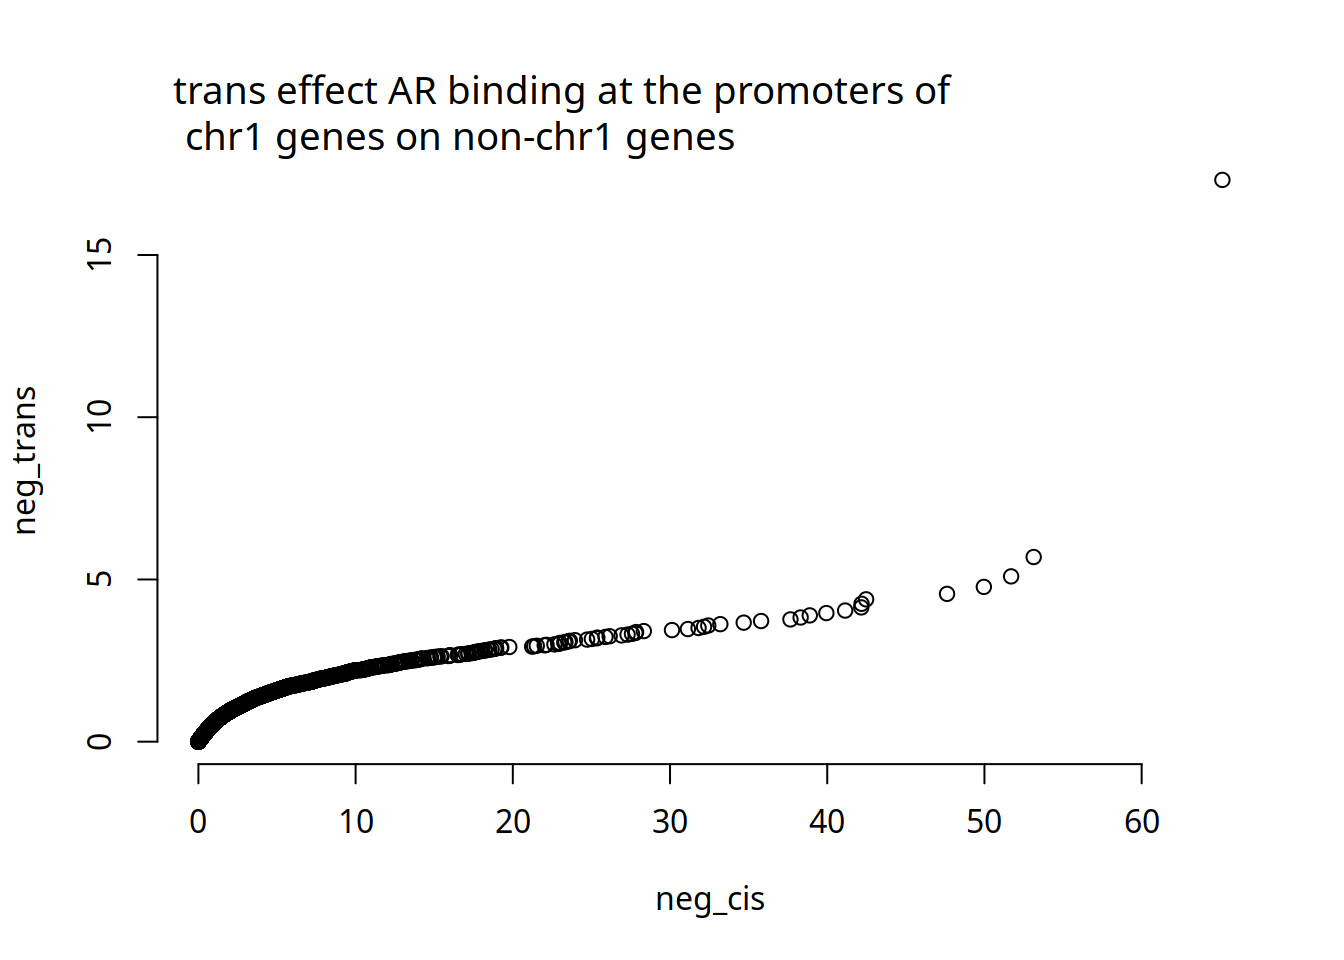
\includegraphics{impact-enformer-modelling_files/figure-pdf/unnamed-chunk-47-1.pdf}

}

\end{figure}

\begin{Shaded}
\begin{Highlighting}[]
\CommentTok{\# dev.copy(png, glue(\textquotesingle{}\{plots\_dir\}/spread{-}of{-}coefficients.png\textquotesingle{}))}
\CommentTok{\# dev.off()}
\end{Highlighting}
\end{Shaded}

\begin{Shaded}
\begin{Highlighting}[]
\CommentTok{\#dev.print(png, glue(\textquotesingle{}\{plots\_dir\}/spread{-}of{-}coefficients{-}except{-}GATA3{-}aggByCenter.png\textquotesingle{}), width=3)}
\CommentTok{\#dev.off()}
\end{Highlighting}
\end{Shaded}




\end{document}
